\chapter{Systematic Uncertainties}

Systematic uncertainty control is very important to and a highlight of this 
high-precision experiment. To achieve a smaller systematic uncertainty, a
combination of fast-control and slow control was employed, which helped us
to eliminate systematic uncertainties brought by the accelerator to the
beam. Except the uncertainty from the machine, another important source
of systematic undertainties come from detection process, namely the 
acceptance function.

\section{Carbon Contamination in PREX-II}

\section{Accptance Function}
The acceptance function is defined as the proportion of detected electrons
over scattered electrons, it is a function of the scattering angle $\theta$:
$$ A(\theta) = \frac{N_{det}(\theta)}{N_{sca}} $$

The acceptance function has another importance: only with the acceptance
function, can we interpret our measurement:
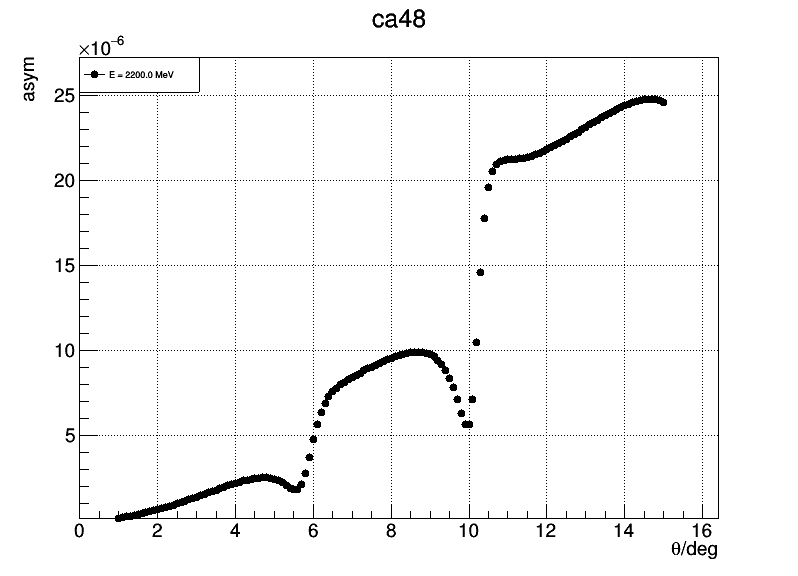
\includegraphics[width=0.5\linewidth]{asym_ca48}
\begin{equation*}
    \langle A \rangle = \frac{\int d\theta \sin\theta A(\theta) \frac{d\sigma}{d\Omega} \epsilon(\theta)}{\int d\theta \sin\theta \frac{d\sigma}{d\Omega} \epsilon(\theta)}
\end{equation*}

The idea is to match simulation with optics data; then we can extract the 
acceptance function from the simulation. For optics data, we have 2 sieves
(which is just a thin steel plane with many holes on it) before the septum.
Because we know each hole position on the sieve, we can therefore reconstruct
the transfrom matrices between target and detector. Which can then be used in
simulation to extract the acceptance function.

For the simulation, we need to identify a few things:
\begin{itemize}
    \item Beam Position
    \item 
\end{itemize}

We will scan through some parameters to find the best model:
\begin{itemize}
    \item Septum current
    \item Collimator shift
    \item Pinch point shift
\end{itemize}

\subsection{Optics Data}
% \subsection{tgt variables}
